\documentclass[oneside]{article}
\title{Exercise 1}
\author{Orgho Anoronyo Neogi}
\date{09 December 2016}
\usepackage{amsmath}
\usepackage{graphicx}
\usepackage{listings}
\lstset{language=java}
\lstset{morekeywords={
    arguments,
    debugger,
    delete,
    eval,
    export,
    false,
    function,
    in,
    let,
    null,
    true,
    typeof,
    var,
    with,
    yield}}
\lstset{deletekeywords={assert, strictfp}}
\usepackage[colorlinks=true]{hyperref}
\begin{document}
\maketitle

\begin{enumerate}
  \item Here are equations that contain trigonometric functions:

  \begin{align*}
    x & = r \cos \psi \\
    y & = r \sin \psi
    \end{align*}

  \item Here is an expression that contains the dot
    product of two vectors:

  \begin{align*}
    \vec{u} \cdot \vec{v} & = \cos \phi \mid \vec{u} \mid \mid \vec{v} \mid
    \end{align*}

  \item Here is an expression that contains the cross
    product of two vectors:

  \begin{align*}
    \mid \vec{u} \times \vec{v} \mid & =
        \sin \phi \mid \vec{u} \mid \mid \vec{v} \mid
    \end{align*}

  \item Here is a matrix:

  \begin{align*}
    \begin{bmatrix}
      m_{00} & m_{01} & m_{02} & m_{03} \\
      m_{10} & m_{11} & m_{12} & m_{13} \\
      m_{20} & m_{21} & m_{22} & m_{23} \\
      m_{30} & m_{31} & m_{32} & m_{33}
      \end{bmatrix}
    \end{align*}

  \item Here is a product of a matrix and a column vector:

  \begin{align*}
    \begin{bmatrix}
      m_{00} & m_{01} & m_{02} & m_{03} \\
      m_{10} & m_{11} & m_{12} & m_{13} \\
      m_{20} & m_{21} & m_{22} & m_{23} \\
      m_{30} & m_{31} & m_{32} & m_{33}
      \end{bmatrix}
    \begin{bmatrix}
      u_0 \\
      u_1 \\
      u_2 \\
      u_3
      \end{bmatrix}
    \end{align*}

  \item Here is a product of a matrix and
      a column vector with the result:

  \begin{align*}
    \begin{bmatrix}
      m_{00} & m_{01} & m_{02} & m_{03} \\
      m_{10} & m_{11} & m_{12} & m_{13} \\
      m_{20} & m_{21} & m_{22} & m_{23} \\
      m_{30} & m_{31} & m_{32} & m_{33}
      \end{bmatrix}
    \begin{bmatrix}
      u_0 \\
      u_1 \\
      u_2 \\
      u_3
      \end{bmatrix}
    & =
    \begin{bmatrix}
      v_0 \\
      v_1 \\
      v_2 \\
      v_3
      \end{bmatrix}
    \end{align*}

  \item Here is a product of a row vector, a matrix, and a column
    vector with the result:

  \begin{align*}
    \begin{matrix}
    \begin{bmatrix}
        u_0 & u_1 & u_2 & u_3
        \end{bmatrix} \\
        \mbox{} \\
        \mbox{} \\
        \mbox{}
        \end{matrix}
    \begin{bmatrix}
      m_{00} & m_{01} & m_{02} & m_{03} \\
      m_{10} & m_{11} & m_{12} & m_{13} \\
      m_{20} & m_{21} & m_{22} & m_{23} \\
      m_{30} & m_{31} & m_{32} & m_{33}
      \end{bmatrix}
    \begin{bmatrix}
      v_0 \\
      v_1 \\
      v_2 \\
      v_3
      \end{bmatrix}
    & = x
    \end{align*}

  \item Here is some JavaScript:

  \begin{lstlisting}{}
    var f = function( u, v ) {
        var r = 1 + Math.sin( 8 * u ) / 10;
        var x = r * Math.cos( v );
        var y = r * Math.sin( v );
        var z = u;

        return new THREE.Vector3( x, y, z );
    }; // f()
    \end{lstlisting}

  \item See this image~\ref{planets}:

  \begin{figure}
  \begin{center}
    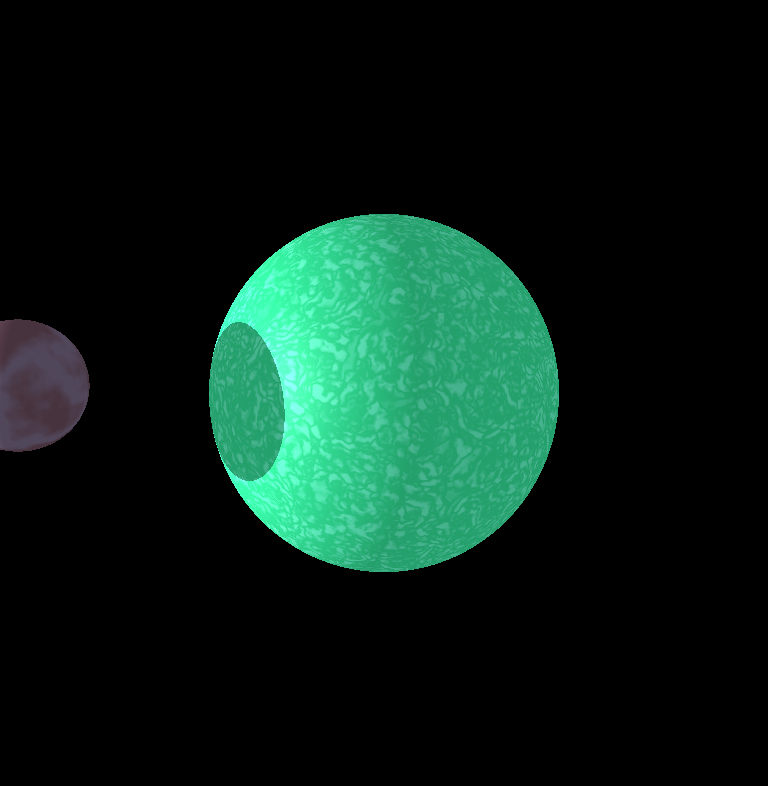
\includegraphics[width=8cm]{planets}
    \end{center}
    \caption{Planets}
    \label{planets}
    \end{figure}

  \end{enumerate}

\end{document}
